% !TEX program = xelatex
% ============================================================
%  2026 年度“策联杯”数学建模精英联赛 B 题参赛论文
%  海上油田人员直升机运载计划编排优化探究
%  编译方式：XeLaTeX
% ============================================================
\documentclass[UTF8,zihao=-4]{ctexart}

% ---------------- 页面设置 ----------------
\usepackage[top=2.5cm,bottom=2.5cm,left=2.5cm,right=2.5cm]{geometry}
\pagestyle{plain}   % 无页眉，页脚中部页码

% ---------------- 数学公式 ----------------
\usepackage{amsmath,amssymb,amsthm}

% ---------------- 图表与代码 ----------------
\usepackage{graphicx}
\usepackage{booktabs}
\usepackage{longtable}
\usepackage{array}
\usepackage{multirow}
\usepackage{float}
\usepackage{caption}
\usepackage{listings}
\usepackage{xcolor}
\usepackage[hidelinks]{hyperref}

% 图片路径：所有插图统一放在 paper/figures/
\graphicspath{{figures/}}

% ---------------- 标题层级 ----------------
\ctexset{
  section       = {format={\zihao{3}\bfseries\centering}, number=\chinese{section}, name={,、}, aftername={}},
  subsection    = {format={\zihao{4}\bfseries}, number=\arabic{section}.\arabic{subsection}, aftername={\quad}},
  subsubsection = {format={\zihao{-4}\bfseries}, number=\arabic{section}.\arabic{subsection}.\arabic{subsubsection}, aftername={\quad}},
}

% 图、表按节编号（图5.1、表2.1）
\numberwithin{figure}{section}
\numberwithin{table}{section}
\renewcommand{\thefigure}{\arabic{section}.\arabic{figure}}
\renewcommand{\thetable}{\arabic{section}.\arabic{table}}

\captionsetup{font=small,labelfont=bf}

% ---------------- 代码样式（附录贴源代码用，加边框） ----------------
\definecolor{codebg}{RGB}{247,247,247}
\lstset{
  basicstyle=\ttfamily\footnotesize,
  backgroundcolor=\color{codebg},
  frame=single,
  rulecolor=\color{gray!40},
  breaklines=true,
  keywordstyle=\bfseries,
  commentstyle=\color{gray},
  tabsize=2,
  columns=fullflexible,
}

\setlength{\parindent}{2em}
\setlength{\emergencystretch}{2em}

\begin{document}

% ============================================================
%  摘要（第 1 页，专用页，不编号）
% ============================================================
\begin{center}
  {\zihao{2}\bfseries 海上油田人员直升机运载计划编排优化探究}\\[1.2em]
  {\zihao{3}\bfseries 摘\quad 要}
\end{center}
\vspace{0.6em}

海上油田生产连续、人员倒班集中，需以直升机承担出海、海返与穿梭三类人员运输。本文针对 3 座陆地机场、52 座海上设施、三种机型与 8 座可加油设施构成的运载系统，在最小化总飞机使用时间的基础上兼顾人员总在途时间、座位利用率与油耗等次要因素，建立了随问题递进的三个模型，并以精确算法求解。

\textbf{针对问题一}（单向出海运输，1600 人），本文将其抽象为多机场、多机型、带容量与燃油约束的单向车辆路径问题（CVRP 变体）。利用需求按设施编号自然分块、架次不跨机场中转与飞机充足三条结构性事实，把问题按机场解耦为三个同构子问题；对单机场子问题采用“机型感知拆分 + 集合划分”模型，将每设施需求拆为“满座份 + 尾数份”，满座份满载单飞、尾数份合并为环游，并以显式枚举 + 整数规划精确求解，燃油约束简化为“相邻加油点间累计距离不超过最大不加油航程”的可行性规则。结果表明，总飞机使用时间 \textbf{15061} 分钟、人员总在途时间 \textbf{131033} 分钟、总架次数 \textbf{88}、总燃油消耗量 \textbf{120920.1} kg、座位利用率 \textbf{49.68\%}；以 85 架次为理论架次数下界，LP 松弛下界 15041 分钟，求解 gap 为 \textbf{0.13\%}。

\textbf{针对问题二}（出海、海返与穿梭联合运输，4000 人），本文将其升级为带同时取送的车辆路径问题（VRPSPD）。核心发现是出海与海返在设施层面高度配对（净差落在 $[-4,+6]$），据此提出“配对往返、穿梭顺路承载”的建模思路：满座部分配对为往返架次使架次数近乎减半，尾数由出海、海返独立合并为环游，穿梭作为环游途中顺路承载的乘客；建立以 OD 对为覆盖对象的集合划分整数规划，以列生成精确求解。结果表明，总飞机使用时间 \textbf{23358} 分钟、人员总在途时间 \textbf{311587} 分钟、总架次数 \textbf{117}、总燃油消耗量 \textbf{176360.6} kg、座位利用率 \textbf{73.01\%}。

\textbf{针对问题三}（带时间要求的多日排班，4000 人 + 24 架飞机），本文在 VRPSPD 之上叠加时间窗与有限机队两重约束。核心发现是任务类型与窗口紧度高度相关：应急处置与增储上产共 400 人窗口落在单天之内、被锁定在窗日且只能小群组直飞，常规倒班与临时任务共 3600 人窗口跨 2--4 天、“哪天飞”成为决策变量，据此提出“紧核单天固定、松壳跨天可选”的分层思路，建立“日级主问题 + 天内排班”两层模型，并按两阶段处理临时任务。结果表明，临时人员满足 \textbf{148} 人（满足率 \textbf{92.5\%}），总飞机使用时间 \textbf{48060} 分钟、人员总在途时间 \textbf{305847} 分钟、总架次数 \textbf{248}、总燃油消耗量 \textbf{373466.3} kg、座位利用率 \textbf{37.16\%}。

\vspace{1em}
\noindent\textbf{关键词：}\textbf{直升机运载计划；车辆路径问题；集合划分；列生成；分层规划；整数规划}

\newpage

% ============================================================
%  一、问题重述
% ============================================================
\section{问题重述}

\subsection{问题背景}

海上油田由多个油气田及配套生产设施构成，生产运行、安全管理、设备维修与后勤保障等环节需要不同专业人员长期驻守，海岗员工到期后集中换班。换班时接班人员出海、离岗人员海返，生产任务与检维修安排还会带来设施之间的穿梭，人员往返主要由直升机运输。本题聚焦这一人员运输系统，包含 3 座陆地机场（A01、A02、A03）与 52 座海上设施（F001--F052），海上设施均位于距海岸 100--250 km 海域，其中 8 座（F006、F011、F018、F024、F031、F038、F044、F050）设有可加油点。人员运输按业务性质分为应急处置、增储上产、常规倒班、临时任务四类，优先级依次递减；将人员自陆地机场送往海上设施称为出海、自设施返回机场称为海返、自一座设施前往另一座称为穿梭。

可用的直升机机型为 T1、T2、T3，主要参数见表~\ref{tab:aircraft}。每个架次从机场满油起飞，到达每一处地点以及最终返回机场时的剩余燃油不得低于该机型最低安全余油量，停靠期间不另计油耗；在可加油设施停靠时可选择是否加油，加油即加满，不加油每次停靠至少 10 分钟、加油至少 20 分钟。不考虑机场、设施与加油站的并发容量限制。

\begin{table}[H]
  \centering
  \caption{三种直升机的主要参数}
  \label{tab:aircraft}
  \begin{tabular}{cccccc}
    \toprule
    机型 & 座位数 & 速度 (km/h) & 油耗 (kg/km) & 油箱容量 (kg) & 最低安全余油量 (kg) \\
    \midrule
    T1 & 12 & 250 & 3.4 & 1000 & 150 \\
    T2 & 16 & 220 & 2.5 & 1150 & 150 \\
    T3 & 19 & 190 & 2.9 & 1600 & 200 \\
    \bottomrule
  \end{tabular}
\end{table}

\subsection{问题提出}

本题的考核目标是飞机使用时间，即一个架次自机场起飞至返回同一机场的时间、含飞行与海上停靠，总飞机使用时间为各架次之和；同时需考虑人员总在途时间与座位利用率两项次要因素，前者指人员自其所乘飞机离开起点至到达终点的总时长，后者指全部航段客座公里与可用座公里之比。需完成以下三个问题：

问题 1：单向出海运输。peopleQ1.csv 给出 1600 条出海需求，不考虑时间窗与业务优先级、飞机数量充足，在最小化总飞机使用时间的基础上尽可能优化座位利用率、油耗等次要因素，输出 q1-routes.csv 与 q1-assignments.csv，并报告总飞机使用时间、人员总在途时间、总架次数、总燃油消耗量、座位利用率五项指标。

问题 2：出海、海返与穿梭联合运输。peopleQ2.csv 给出 4000 条出海、海返与穿梭需求，同样不考虑时间窗与优先级、飞机充足，在最小化总飞机使用时间的基础上尽可能优化其他因素，输出 q2-routes.csv 与 q2-assignments.csv，并报告五项指标。

问题 3：带时间要求的多日排班。peopleQ3.csv 在问题 2 基础上为每名人员增加最早登机时刻、最晚到达时刻与任务类型，需求时间落在 2026-08-03 至 08-10 之间。使用表~\ref{tab:fleet} 所列 24 架飞机，机场运营时段内可在 06:00--18:00 起飞、不得晚于 20:00 返回、不得在海上过夜，同一飞机完成一个架次后至少经过 30 分钟机场周转。临时任务可因减少开销而取消：先在不考虑临时任务时编排得到总飞机使用时间，再在不超过该时间的条件下尽可能多地满足临时需求，输出 q3-routes.csv 与 q3-assignments.csv，并报告临时满足情况与五项指标。

\begin{table}[H]
  \centering
  \caption{排班可用直升机（表 3）}
  \label{tab:fleet}
  \begin{tabular}{ccccc}
    \toprule
    机场 & T1 & T2 & T3 & 合计 \\
    \midrule
    A01 & 3 & 3 & 2 & 8 \\
    A02 & 2 & 4 & 2 & 8 \\
    A03 & 2 & 3 & 3 & 8 \\
    \midrule
    合计 & 7 & 10 & 7 & 24 \\
    \bottomrule
  \end{tabular}
\end{table}

% ============================================================
%  二、问题分析
% ============================================================
\section{问题分析}

三个问题构成一条由简到繁、逐层递进的建模链，其本质是同一运输系统在不同约束维度下的车辆路径问题（VRP）变体。我们沿同一主线展开：先观察数据、找出结构性特征，再据此分解问题、构造候选解，最后选择规模上可行、质量上可评估的算法。

\textbf{数据特征}：问题一数据 peopleQ1.csv 共 1600 条出海需求，按出发地分为 A01、A02、A03 三类指定机场与 LAND四类，目的地覆盖全部 52 座海上设施。图~\ref{fig:q1od} 给出出发地 $\times$ 目的地的需求量热力矩阵，其最显著的特征是严格的块对角结构——A01、A02、A03 的乘客分别只落在 F001--F017、F018--F035、F036--F052 三段、彼此零交叉，本文据此提出三机场可无损失解耦；LAND 乘客虽覆盖全部设施，但其逐设施分布仍与上述三段自然对应，故按设施编号分块即可将 LAND 乘客固定归属最近机场，将整个问题拆解为三个子问题。并且这一特点在问题二，三中也成立。

\begin{figure}[H]
  \centering
  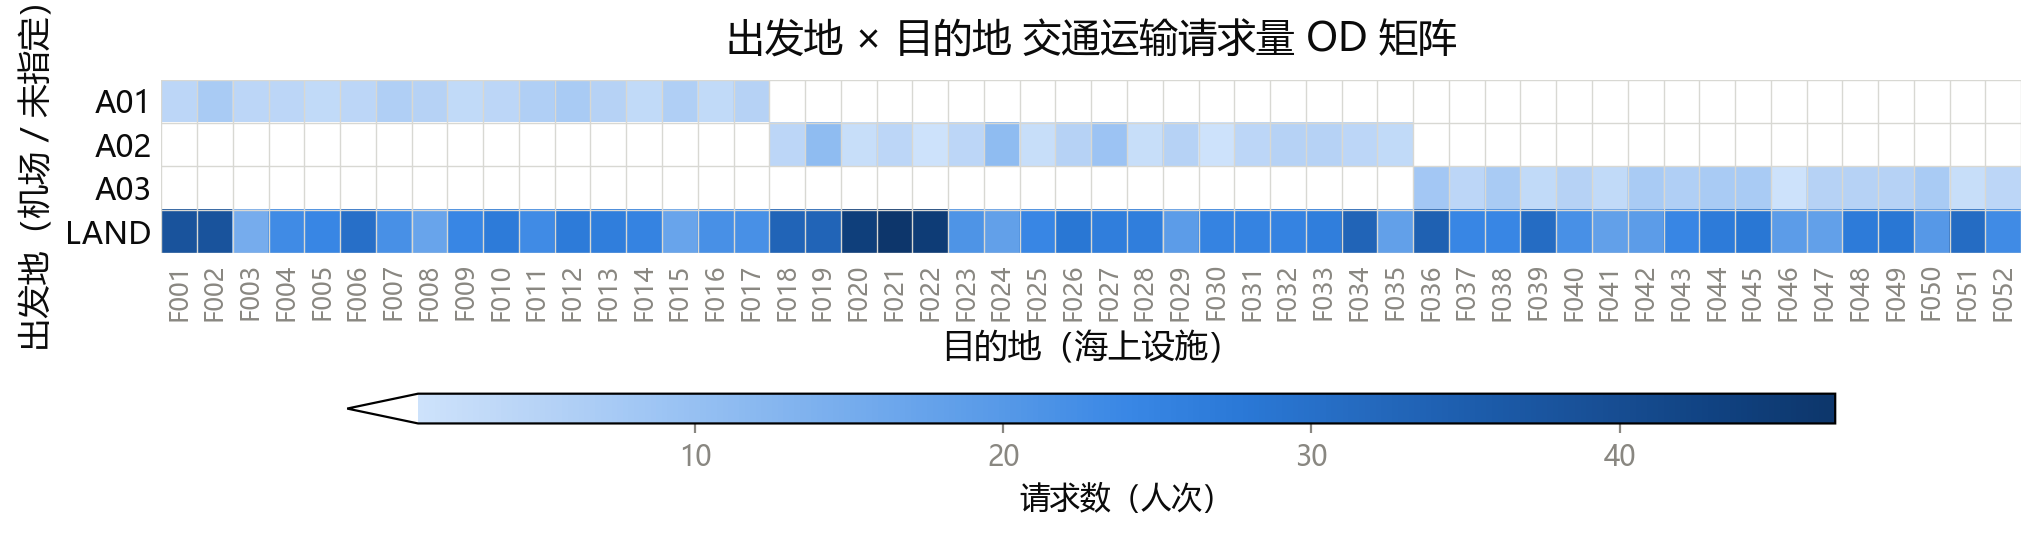
\includegraphics[width=0.92\textwidth]{question1_OD矩阵热力图.png}
  \caption{问题一 OD 需求矩阵热力图（出发地 $\times$ 目的地，呈块对角结构）}
  \label{fig:q1od}
\end{figure}

\subsection{问题一}

问题一只有出海单向运输、人员只下不上，是带容量与燃油约束的单向 CVRP。数据统计揭示两条决定性结构特征：

三机场严格解耦：指定机场的人员天然落在其所属设施号段——A01 服务 F001--F017、A02 服务 F018--F035、A03 服务 F036--F052；穿梭 OD 全部位于同一区块内，跨机场人数为 0。再结合架次不跨机场中转、飞机数量充足的题设，按设施分块即可把总问题分解为三个互不相干的子问题，且不损失任何最优性。

“满座 + 尾数”需求拆分：单机最多 19 座而每设施需求 19--51 人，任一设施的需求都须拆分给多个架次共同运送。既然满载直飞已是这部分人员最快的运送方式，就把每设施需求拆成“满座份 + 尾数份”：满座份满载单飞、直接固化为成本；尾数份跨设施合并为环游、一次飞多设施以省去多次机场往返。这样优化空间就被压缩到“尾数合并”这一个环节，而合并只受座位数不超过 19 与停靠次数不超过 5 的双重约束。

\subsection{问题二}

问题二加入海返与穿梭，同一架次既承载出海的到达又承载海返的出发，机上人数沿环游先减后增、不再单调，且每名人员须由同一架次直送终点、不得换乘，升级为带同时取送的 VRPSPD。其关键结构特征是：

出海与海返高度配对：对问题二数据的预分析显示，各设施出海与海返人数之差落在 $[-4,+6]$、48/52 个设施在 $\pm3$ 以内（图~\ref{fig:q2netdiff}），即“送去多少人、几乎接回多少人”。受此启发，把满座部分配对为往返架次，去程满载送达、返程满载接回，一个架次兼负两程、使架次数近乎减半；只有真正新增的穿梭客流与未配对的少量尾数需要额外运力。

\begin{figure}[H]
  \centering
  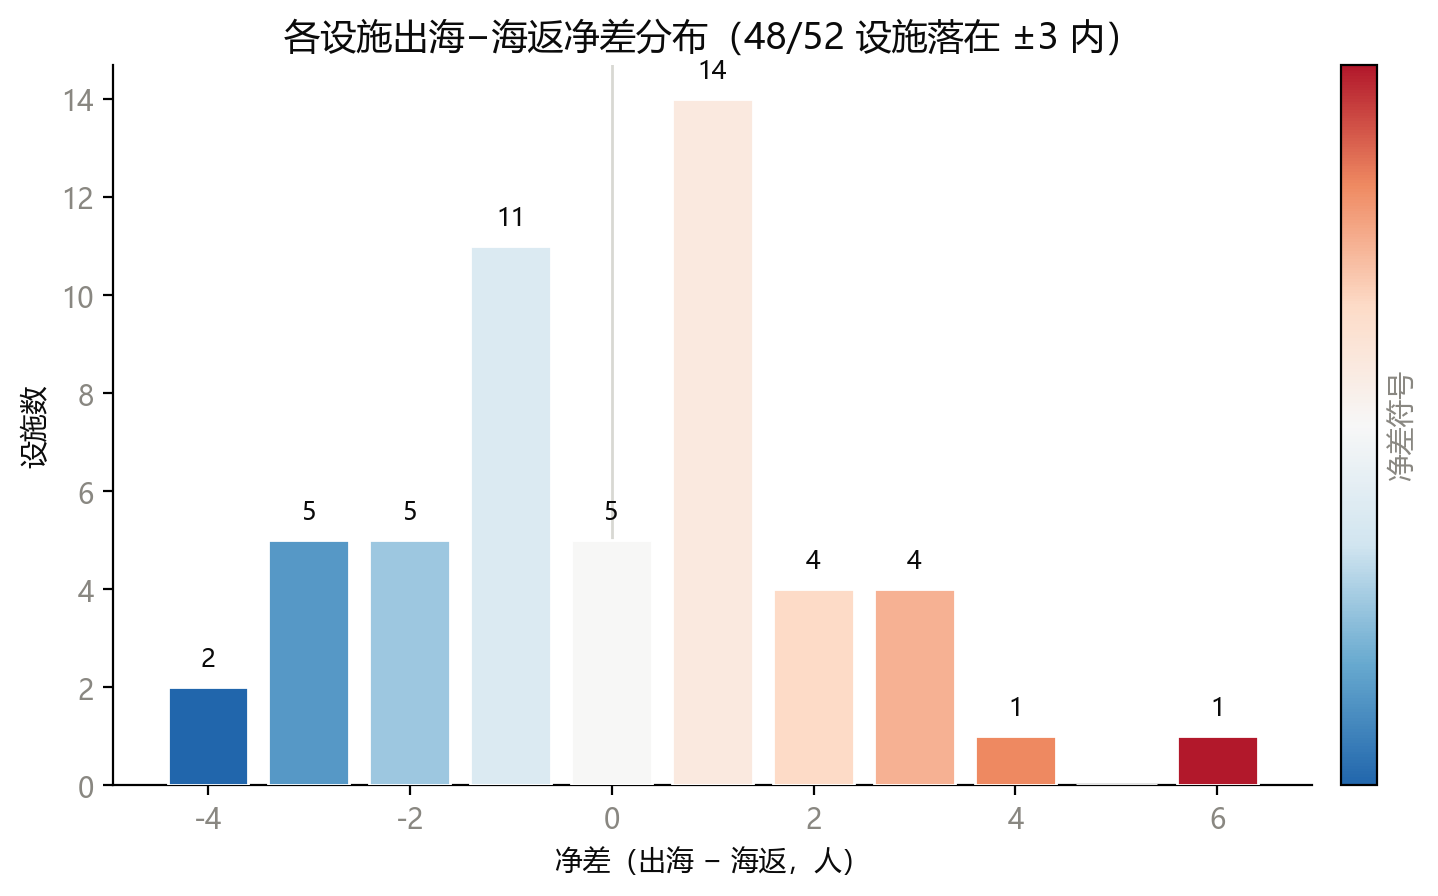
\includegraphics[width=0.60\textwidth]{问题二_净差直方图.png}
  \caption{问题二各设施出海$-$海返净差分布（48/52 设施在 $\pm3$ 内，据此配对往返）}
  \label{fig:q2netdiff}
\end{figure}

\subsection{问题三}

问题三在问题二路由结构不变的基础上，叠加时间窗与有限机队两重约束，是 VRPTW 与机队调度的结合。其关键结构特征是：

任务类型与窗口紧度高度相关：应急处置与增储上产共 400 人的窗口全部落在单天之内，最短者不足半小时，其航班被迫落在窗日、只能小群组直飞；常规倒班与临时任务共 3600 人的窗口跨 2--4 天，“哪天飞”才是真正的决策变量（图~\ref{fig:q3window}）。据此把需求分为紧核 400 人与松壳 3600 人两层，前者单天固定、后者跨天可选，其求解顺序恰与题目“应急处置 $\to$ 增储上产 $\to$ 常规倒班 $\to$ 临时任务”的优先级一致。

\begin{figure}[H]
  \centering
  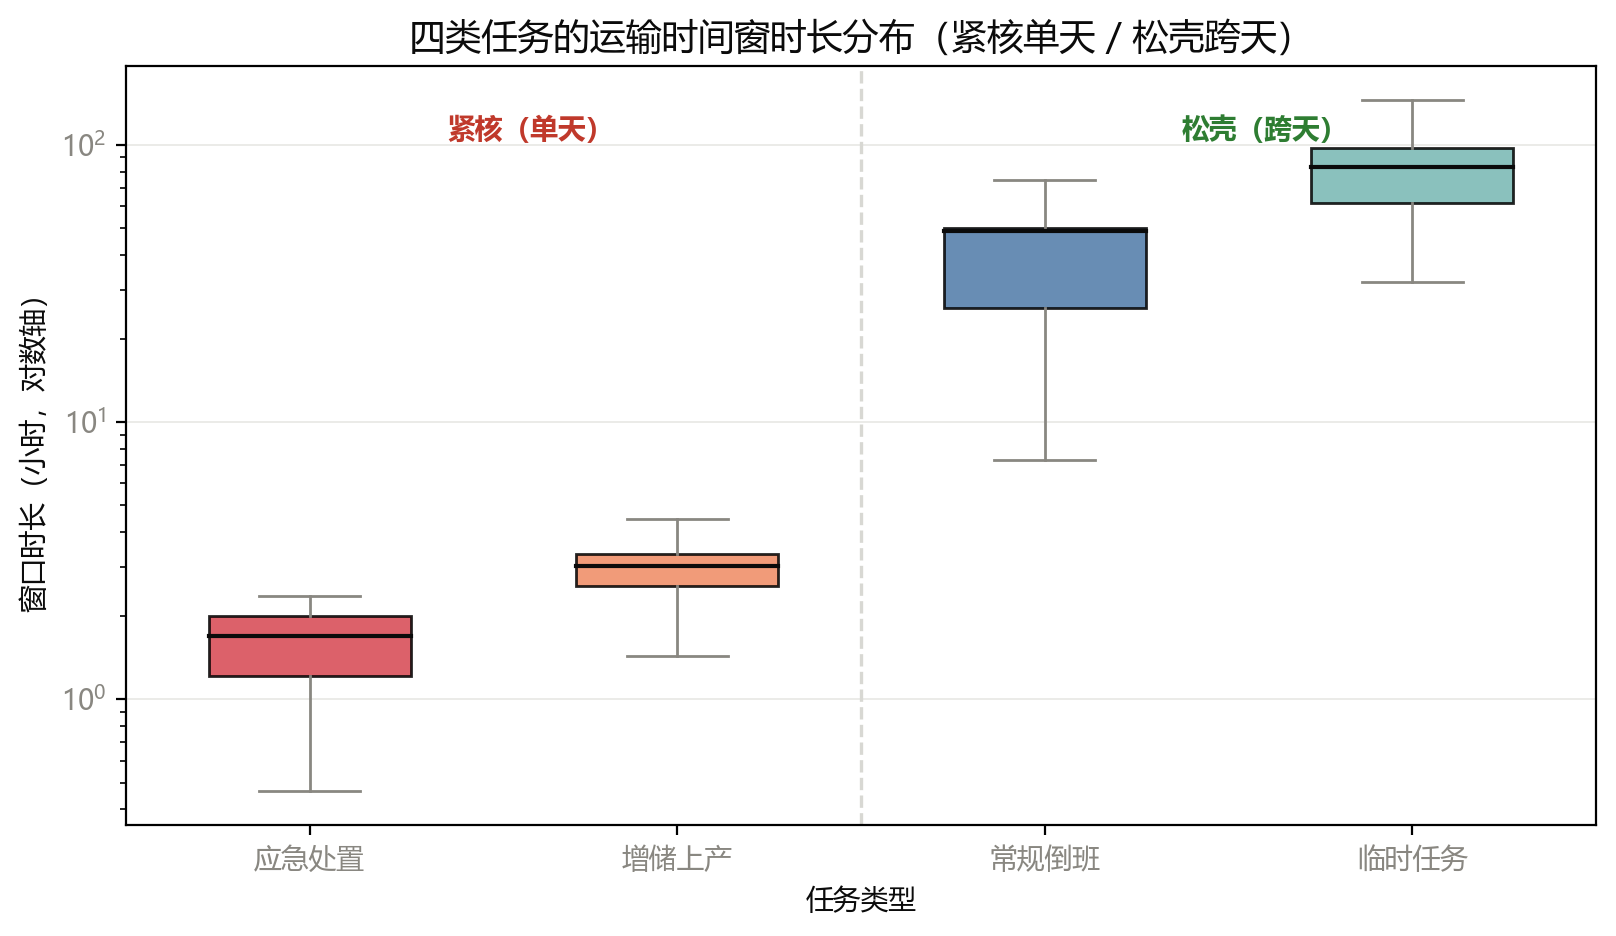
\includegraphics[width=0.62\textwidth]{问题三_窗口时长箱线图.png}
  \caption{问题三四类任务的运输时间窗时长分布（紧核单天 / 松壳跨天）}
  \label{fig:q3window}
\end{figure}

% ============================================================
%  三、模型假设
% ============================================================
\section{模型假设}

\begin{enumerate}
  \item 人员上下机与地面调度时间忽略不计，仅计飞行时间与海上停靠时间；
  \item 飞行速度与单位距离油耗不随载客量变化，满载与空载航速、油耗相同；
  \item 机场、海上设施与加油站的并发容量无需考虑，故忽略其限制；
  \item 停靠时间取最小值：不加油 10 分钟、加油 20 分钟，允许等待延长；所有时间向上取整到整数分钟；
  \item 距离矩阵对称且满足三角不等式，可直接用于 TSP 求解；
  \item 每名人员由同一架次自起点直送终点、中途不得换乘；
  \item 架次自某机场起飞、最终返回同一机场，不跨机场中转。
\end{enumerate}

% ============================================================
%  四、符号说明
% ============================================================
\section{符号说明}

\begin{longtable}{p{3.4cm}@{\qquad}p{10.2cm}}
  \caption{主要符号说明}\label{tab:notation}\\
  \toprule
  符号 & 含义 \\
  \midrule
  \endfirsthead
  \toprule
  符号 & 含义 \\
  \midrule
  \endhead
  $\mathcal{A}=\{A01,A02,A03\}$ & 机场集合 \\
  $\mathcal{F}=\{F001,\dots,F052\}$ & 海上设施集合，$|\mathcal{F}|=52$ \\
  $\mathcal{R}\subset\mathcal{F}$ & 可加油设施集合（8 个） \\
  $\mathcal{M}=\{T1,T2,T3\}$ & 机型集合 \\
  $\mathcal{D}=\{1,\dots,7\}$ & 规划期天数集合（问题三） \\
  $\mathcal{T}$ & 任务类型集合（问题三） \\
  $c_m, v_m, f_m, U_m, \underline{u}_m$ & 机型 $m$ 的座位数、速度(km/h)、油耗(kg/km)、油箱容量(kg)、最低安全余油量(kg) \\
  $\bar d_m=(U_m-\underline{u}_m)/f_m$ & 机型 $m$ 的最大不加油航程(km) \\
  $d_{uv}$ & 节点 $u,v$ 间距离(km) \\
  $q_d^{\mathrm{out}}, q_d^{\mathrm{ret}}, q^{\mathrm{sh}}_{(i,j)}$ & 设施 $d$ 出海、海返人数及穿梭 OD $(i,j)$ 人数 \\
  $D_{(i,j)}^{\tau}$ & OD $(i,j)$ 上任务类型 $\tau$ 的需求人数（问题三） \\
  $r$、$a_r$、$m_r$、$S_r$ & 架次（列）及其起飞机场、机型、访问设施子集 \\
  $d_r^{\mathrm{TSP}}$、$T_r$、$k$、$g_r$ & 架次 $r$ 的环游距离、总时间、海上停靠次数、加油次数 \\
  $n_{r,(i,j)}$ & 架次 $r$ 承载 OD $(i,j)$ 的人数 \\
  $\lambda_r$（$\lambda_{r,d}$） & 架次 $r$（第 $d$ 天）的使用次数（整数变量） \\
  $y_s$、$n_s$、$p_s$ & 拆分方案 $s$ 的选择变量、满座份数、尾数份人数（问题一） \\
  $P_r, F_r, E_r$ & 架次 $r$ 的人员总在途时间、油耗、空座$\cdot$距离（次指标系数） \\
  $P_0,F_0,E_0$；$w_P,w_F,w_\eta$ & 无量纲化基准；次指标权重（$w_P+w_F+w_\eta=1$） \\
  $\eta$ & 座位利用率 \\
  $z_{LP}, z_{IP}$ & 集合划分 IP 的 LP 松弛下界、整数最优值 \\
  \bottomrule
\end{longtable}

% ============================================================
%  五、模型的建立与求解
% ============================================================
\section{模型的建立与求解}

\subsection{问题一}

\subsubsection{三机场解耦与单机场子问题的建立}

问题一需同时决定每名乘客的起飞机场、每架次访问的设施集合与顺序、机型以及加油方案，规模大且 NP-hard，直接整体求解不可行。我们转而寻找可分性，观察到三条结构性事实：人员不可换乘、架次不跨机场中转、飞机数量充足。由前两条，任一架次自始至终只服务其起飞机场周边的设施；由第三条，机场间无需共享资源。故只要每名乘客的起飞机场被确定，总问题即退化为三个互不相干、结构完全相同的单机场子问题：

\begin{equation}
  \min \sum_{a\in\mathcal{A}} \mathrm{VSP}(a)
\end{equation}

其中 $\mathrm{VSP}(a)$ 为机场 $a$ 的单机场航线编排子问题。唯一障碍是 1353 名 LAND 乘客没有指定起飞机场，若把机场选择留作决策变量，三机场将通过 LAND 乘客相互耦合。因此，下一小节借助“设施沿海岸线线性排列、编号与机场位置一致”的地理结构，把 LAND 乘客按设施分块固定归属机场，从而把机场选择退化为固定参数，完成分解。

\subsubsection{LAND 乘客的机场归属与三机场解耦}

设施编号 F001--F052 沿海岸线自北向南线性排列，与三机场位置分布一致，故按编号等分为三段即可同时兼顾“就近”与“均衡”：

\begin{equation}
  \sigma(d)=\begin{cases}
    A01, & d\in\{F001,\dots,F017\}\\
    A02, & d\in\{F018,\dots,F035\}\\
    A03, & d\in\{F036,\dots,F052\}
  \end{cases}
\end{equation}

三段负载分别为 499/598/503 人，接近均衡。将设施 $d$ 的全部需求统一由 $\sigma(d)$ 服务，则各机场的设施集合与人数均为固定参数 $\mathcal{F}_a=\{d:\sigma(d)=a\}$、$q_{d,a}=q_d\,\mathbb{1}[\sigma(d)=a]$。由数据统计，指定机场乘客的分布与式 (2) 的分块完全一致，故 $\sigma(d)$ 对所有乘客都是其天然归属。

\subsubsection{超容量设施需求的多机型拆分}

同一设施的需求可能由任一机型运送，且拆分方式决定后续尾数合并的空间（需求被拆分给多架次共同运送，属可拆分配送问题\cite{ref:sd}）。因此把“机型 $\times$ 拆分方式”的每种可能都生成一个候选拆分方案 $s=(m_s,n_s,p_s)$，把机型选择与拆分的耦合交给最终 IP 择优：

\begin{equation}
  n_s=\left\lfloor\frac{q_d}{c_{m_s}}\right\rfloor,\qquad p_s=q_d-c_{m_s}\,n_s
\end{equation}

其中 $n_s$ 为满座架次数、每架满载 $c_{m_s}$ 人，$p_s$ 为拆不尽的尾数份人数且 $0\le p_s<c_{m_s}$。例如 $q_d=29$：T3 得 $(19,1,10)$、T2 得 $(16,1,13)$、T1 得 $(12,2,5)$，三种方案构成候选集合 $D_d$。

\subsubsection{满载份的独立运送与固定时间成本}

满座份人数恰等于座位数，满载单飞已是该部分人员的最快运送方式，再并入其他设施只会增加飞行与停靠，故满座架次不参与合并、直接固化为固定成本：

\begin{equation}
  T^{\text{满}}(d,m)=\frac{2\,d_{\sigma(d),d}}{v_m}+10+10\,g
\end{equation}

其中 $g\in\{0,1\}$ 表示该满座架次是否加油，由燃油判据确定；若该机型无法直达，即往返超过最大不加油航程且 $d$ 非可加油设施，则此方案剔除。

\subsubsection{尾数份的跨设施合并运送}

真正需要决策的只剩各设施的尾数份。以 $(d,m_s)$ 标识一条尾数份，即设施 $d$ 在机型 $m_s$ 下的尾数、人数 $p_s$，于是一个架次可把若干不同设施的尾数份合并为一条“机场 $\to$ 若干设施 $\to$ 机场”的环游。设尾数合并架次 $r$ 含尾数份集合 $\Theta_r$、访问设施集合 $S_r$、机型 $m_r$，须满足

\begin{equation}
  \sum_{(d,m_s)\in\Theta_r} p_s \le c_{m_r},\qquad |S_r|\le 5
\end{equation}

即总人数不超过座位数、海上停靠不超过 5 次，且同一设施至多出现一条尾数份。其成本为

\begin{equation}
  T_r=\frac{d_r^{\mathrm{TSP}}}{v_{m_r}}+10\,|S_r|+10\,g_r
\end{equation}

其中 $d_r^{\mathrm{TSP}}$ 为访问 $S_r$ 中设施的最短环游距离，由不超过 5 个点的 TSP 求得。

\subsubsection{覆盖全部需求的架次选择整数规划}

为每个拆分方案设 0-1 变量 $y_s$、为每条尾数合并架次设整数变量 $\lambda_r$，得集合划分 IP：

\begin{equation}
  \min \sum_{d}\sum_{s\in D_d} y_s\,n_s\,T^{\text{满}}(d,m_s)+\sum_{r}T_r\,\lambda_r
\end{equation}

\begin{equation}
  \text{s.t.}\quad \sum_{s\in D_d} y_s=1,\quad \forall d\in\mathcal{F}_a
\end{equation}

\begin{equation}
  \sum_{r:\ (d,m_s)\in\Theta_r}\lambda_r = y_s,\quad \forall d,\ \forall s\in D_d,\ p_s>0
\end{equation}

\begin{equation}
  y_s\in\{0,1\},\qquad \lambda_r\in\mathbb{Z}_+
\end{equation}

式 (7) 第一项为满座架次固定时间、第二项为尾数合并架次时间；式 (8) 保证每设施恰选一个拆分方案；式 (9) 把所选方案的尾数份与其运载架次对齐。容量与停靠上限已内化于列定义（式 (5)），无需在 IP 中显式写出。

\subsubsection{最小化总航时并兼顾次指标的分层目标}

题目要求“在最小化总飞机使用时间的基础上尽可能优化次要因素”——这是一个典型的分层（字典序）结构：主目标优先，次要因素只在主目标最优的解集内起区分作用。据此三问统一采用分层加权目标：第一层最小化总飞机使用时间，对应式 (7)；第二层在航时最优解集内对油耗与座位利用率加权取优。设第一层最优航时 $T^*$，第二层为

\begin{equation}
  \min\ \Big[w_F\frac{F}{F_0}+w_\eta\frac{E}{E_0}\Big]
  \qquad\text{s.t.}\quad \sum_{d,s}y_s n_s T^{\text{满}}(d,m_s)+\sum_r T_r\lambda_r=T^*,\quad \text{式}(8)\text{--}(10)
\end{equation}

其中 $F$、$E$ 为总油耗与总空座$\cdot$距离，空座$\cdot$距离是座位利用率的线性代理；$F_0,E_0$ 为无量纲化基准，权重 $w_F+w_\eta=1$ 由层次分析法确定并经敏感性分析验证。由于问题一架次结构由容量与燃油约束主导，第二层次指标对总航时的影响极小，故以第一层最优解报告各项指标。

\subsubsection{架次燃油可行性与中途加油点插入}

燃油约束是航线的可行性条件而非目标项：要求每架次全程剩余油量不低于安全余油。记架次路线为 $a=s_0\to s_1\to\cdots\to s_k\to s_{k+1}=a$，飞机满油起飞，到达每站后剩余油量递推：

\begin{equation}
  u_i=\begin{cases}
    U_m, & s_i\in\mathcal{R}\ \text{且在该站加油}\\
    u_{i-1}-f_m\,d_{s_{i-1},s_i}, & \text{否则}
  \end{cases}
\end{equation}

可行性要求每一站以及返回机场处 $u_i\ge\underline{u}_m$。由于加油即加满，式 (12) 等价于：任意两个相邻加油点以及起降机场之间的累计飞行距离不超过最大不加油航程 $\bar d_m$。三种机型 $\bar d_{T1}=250$、$\bar d_{T2}=400$、$\bar d_{T3}\approx483$ km；A03 南端的 F037--F052 距机场 243--403 km、往返超 T3 航程，必须利用可加油设施中途加油。因此，对超航程架次，在其间就近插入 $\mathcal{R}$ 加油点即可修复。

\subsubsection{单机场子问题的精确求解与解质量评估}

解耦后每机场仅 17--18 个设施，首选是显式枚举：只要候选架次能全部列出，集合划分 IP 即可直接精确求解。故采用“显式枚举候选 + 集合划分整数规划”\cite{ref:ilp}精确求解，流程为：(1) 生成拆分候选与满座架次；(2) 深度优先回溯枚举尾数合并架次，剪枝条件为累计人数不超过 19、停靠不超过 5、同一设施至多一条尾数份；(3) 构建并求解集合划分 IP，由 CBC 精确求解；(4) 燃油逐列校验与加油点插入修复；(5) 以 LP 松弛下界评估解质量。以拥有 17 座设施的 A01 为例，尾数合并组合数上界为 $\sum_{k=1}^{5}\binom{17}{k}3^k\approx1.7\times10^6$，经“人数 $\le19$”剪枝后实际列数仅数千至数万，完全可枚举。

\subsubsection{问题一的求解结果与指标分析}

用上述模型与算法求解，得到问题一的完整运载计划，核心指标见表~\ref{tab:q1res}，航线网络见图~\ref{fig:q1net}。

\begin{table}[H]
  \centering
  \caption{问题一五项指标与解质量}
  \label{tab:q1res}
  \begin{tabular}{lcc}
    \toprule
    指标 & 数值 & 说明 \\
    \midrule
    总飞机使用时间 & 15061 min（251.0 h） & 主目标 \\
    人员总在途时间 & 131033 min（2183.9 h） & 次指标 \\
    总架次数 & 88 & 满座 80、尾数合并 8 \\
    总燃油消耗量 & 120920.1 kg & 次指标 \\
    座位利用率 & 49.68\% & 客座公里/可用座公里 \\
    \midrule
    加油次数 & 38 & 中途加油停靠 \\
    LP 松弛下界 & 15041 min & — \\
    最优性 gap & 0.13\% & $(z_{IP}-z_{LP})/z_{LP}$ \\
    求解耗时 & 100.9 s & 单机场汇总 \\
    \bottomrule
  \end{tabular}
\end{table}

\begin{figure}[H]
  \centering
  
\includegraphics[width=0.62\textwidth]{问题一_航线网络图.png}
  \caption{问题一航线网络（三机场分块，88 架次；满座直飞细线、尾数环游粗线）}
  \label{fig:q1net}
\end{figure}

结果分析：总飞机使用时间为 15061 分钟（约 251.0 小时），由 88 个架次完成，平均每架次载客约 $1600/88\approx18.2$ 人。座位利用率为 49.68\%，反映出“满座份满载单飞 + 尾数份合并环游”的拆分策略在缩短总时间与提升利用率之间的折中。求解 gap 仅为 0.13\%（LP 下界 15041 分钟），说明所得整数解与理论下界几乎一致。总加油次数为 38 次，对应远端设施（尤其 A03 南端 F037$\sim$F052 段）超航程架次的中途加油需求。

\subsection{问题二}

\subsubsection{出海与海返配对、穿梭顺路承载的建模思路}

与问题一相比，问题二的本质差异在于：人员需求是包含起点终点的 OD 对，而非“送到即可”，每名人员由同一架次从起点直送终点、不换乘；载荷剖面非单调，设施上既有下机又有上机、机上人数先降后升。因此问题二属于带同时取送的车辆路径问题（VRPSPD）\cite{ref:toth}。

通过统计问题二的数据（见表~\ref{tab:q2data}），得到两条关键发现：出海与海返在设施层面高度配对，穿梭均为同一区块内短途、每 OD 仅 9--19 人。据此提出“配对往返、穿梭顺路承载”的建模思路——出海与海返的满座部分配对为往返架次，去程满载送达、返程满载接回，使架次数近乎减半；不满整座的尾数由出海、海返各自独立合并为环游运送；穿梭人数之少，环游顺路即可带走、无需单独开辟架次。由此问题二在容量结构上退化为问题一，真正新增的仅是海返与穿梭两类客流。

\begin{table}[H]
  \centering
  \caption{问题二数据特征}
  \label{tab:q2data}
  \begin{tabular}{ll}
    \toprule
    项目 & 结论 \\
    \midrule
    需求规模 & 4000 人，出海 1600、海返 1600、穿梭 800 \\
    设施净差 $q^{\mathrm{out}}-q^{\mathrm{ret}}$ & 落在 $[-4,+6]$，48/52 设施在 $\pm3$ 以内 \\
    穿梭 OD & 56 对，均在同区块内短途，每 OD 9--19 人 \\
    跨机场人数 & 0，三机场解耦不产生任何损失 \\
    \bottomrule
  \end{tabular}
\end{table}

\subsubsection{三类需求的拆分与候选架次的构造}

出海与海返两个方向各自独立套用问题一“满座 + 尾数”拆分。满座部分：设施 $d$ 对机型 $c$ 有 $\lfloor q_d^{\mathrm{out}}/c\rfloor$ 个出海满座与 $\lfloor q_d^{\mathrm{ret}}/c\rfloor$ 个海返满座，因出海与海返人数接近，可配成 $\min(\lfloor q_d^{\mathrm{out}}/c\rfloor,\lfloor q_d^{\mathrm{ret}}/c\rfloor)$ 个往返满座加 $\big|\lfloor q_d^{\mathrm{out}}/c\rfloor-\lfloor q_d^{\mathrm{ret}}/c\rfloor\big|$ 个单向满座。尾数部分：出海尾数份 $\{q_d^{\mathrm{out}}\bmod c\}$ 与海返尾数份 $\{q_d^{\mathrm{ret}}\bmod c\}$ 各自独立、不绑定。穿梭部分：每 OD 仅 9--19 人、不超过 19 座，不做满座拆分，作为按需部分承载量 $h_{(i,j)}\in[0,q^{\mathrm{sh}}_{(i,j)}]$ 顺路承载。

一条尾数合并列 $r$ 由「机型 $m_r$ + 有向顺序 $S_r=(s_1,\dots,s_k)$ + 每站出海尾数 $d_t$、海返尾数 $p_t$（各自独立）+ 穿梭承载 $\{h_{(i,j)}\}$」确定。设第 $t$ 站下机 $d_t$ 人、上机 $p_t$ 人，穿梭在对应两站间上下，则逐弧载荷为

\begin{equation}
  L_0=\sum_{t=1}^{k}d_t,\qquad
  L_t=\sum_{u>t} d_u+\sum_{u\le t} p_u+\sum_{i\le t<j} h_{(s_i,s_j)}\quad(t=1,\dots,k)
\end{equation}

列 $r$ 须满足四类可行条件：峰值载荷不超过座位数，即 $\max_{0\le t\le k}L_t\le c_{m_r}$；穿梭 $i$ 须在 $j$ 之前被访问；停靠次数 $k\le5$；燃油可行条件与问题一相同。其 OD 覆盖与成本为

\begin{equation}
  n_{r,(a_r,s_t)}=d_t,\quad n_{r,(s_t,a_r)}=p_t,\quad n_{r,(i,j)}=h_{(i,j)}
\end{equation}

\begin{equation}
  T_r=\frac{d_r^{\mathrm{TSP}}}{v_{m_r}}+10k+10g_r,\qquad
  F_r=d_r^{\mathrm{TSP}}\cdot f_{m_r},\qquad
  E_r=\sum_{\text{seg}\in r}(c_{m_r}-L_{r,\text{seg}})d_{\text{seg}}
\end{equation}

\subsubsection{覆盖全部出行需求的架次选择模型}

问题二中每名人员须由起点直送终点，覆盖对象从“把人送到设施”变为 OD 对；同一 OD 的人员对系统完全等价、可以互换，故按 OD 聚合人数建模、无需逐人设变量。目标仍沿分层加权结构：

\begin{equation}
  \min\ T=\sum_{r\in\Omega} T_r\lambda_r
\end{equation}

\begin{equation}
  \text{s.t.}\quad \sum_{r\in\Omega} n_{r,(i,j)}\lambda_r=D_{(i,j)},\quad\forall(i,j)
\end{equation}

\begin{equation}
  \lambda_r\in\mathbb{Z}_+
\end{equation}

设第一层最优航时 $T^*$，第二层在航时最优解集上：

\begin{equation}
  \min\ \sum_{r\in\Omega}\Big(w_F\frac{F_r}{F_0}+w_\eta\frac{E_r}{E_0}\Big)\lambda_r
  \qquad\text{s.t.}\ \ \sum_{r\in\Omega}T_r\lambda_r=T^*,\ \ \text{式}(16)(17)
\end{equation}

其中 $F_r=d_r^{\mathrm{TSP}}f_{m_r}$ 为列油耗、$E_r$ 为列空座$\cdot$距离，其值越小利用率越高；$F_0,E_0$ 为无量纲化基准，权重 $w_F+w_\eta=1$。与问题一的 $y_s$ 主问题不同，此处拆分约束内化到列生成中，覆盖式主问题更灵活、允许跨机型混合覆盖。

\subsubsection{大规模候选架次下的列生成求解}

问题二的尾数拆开使尾数份约翻倍、穿梭部分承载使选项约增至 8 倍，完整列数从问题一的数千至数万暴涨到 $10^7\sim10^8$ 量级，预枚举不可行。这促使把求解方式升级为列生成\cite{ref:cg,ref:primer}：主问题仍取集合划分形式，但维护一个只含少量列的受限主问题，以覆盖约束的对偶价为“价格信号”引导搜索、按需生成最可能改进目标的列——定价子问题按对偶价通过 DFS 搜索生成负约化成本列。按需生成在概念上是“枚举的惰性版本”：绝大多数永远无用的列自始至终不被显式构造。

两阶段框架：阶段一解式 (16)(17) 的 $\min T$，列生成收敛得 LP 下界，再对受限主问题 CBC 分支定界得整数最优航时 $T^*$；阶段二加时间固定约束 $\sum_r T_r\lambda_r=T^*$、目标换为式 (19)，重跑列生成 + CBC。每阶段内部流程相同：初始受限主问题只含满座列与每设施一条单尾数列，先解 LP 取对偶价，再由 DFS 定价子问题产生负约化成本列，迭代至无负列，最后 CBC 整数化。

列 $r$ 的约化成本为

\begin{equation}
  \bar c_r=T_r-\sum_{(i,j)}n_{r,(i,j)}\pi_{(i,j)}
  =\frac{d_r^{\mathrm{TSP}}}{v_{m_r}}+10k+10g_r-\sum_{t}\big(d_t\pi^{\mathrm{out}}_{s_t}+p_t\pi^{\mathrm{ret}}_{s_t}\big)-\sum_{(i,j)}h_{(i,j)}\pi^{\mathrm{sh}}_{(i,j)}
\end{equation}

其中 $\pi^{\mathrm{out}}_d,\pi^{\mathrm{ret}}_d,\pi^{\mathrm{sh}}_{(i,j)}$ 为出海、海返、穿梭覆盖约束的对偶价。定价子问题采用深度优先搜索 + 约化成本下界剪枝：枚举 $\le5$ 设施的访问顺序，逐站独立选取出海/海返尾数份与穿梭承载，当“已定部分 + 剩余下界”$\ge0$ 时回退，从而保证不遗漏任何负约化成本列，又不必展开完整 $10^8$ 列空间。列生成收敛处的 LP 最优给出下界 $z_{LP}$，整数解由受限主问题 CBC 分支定界求取，gap 以 $(z_{IP}-z_{LP})/z_{LP}$ 报告。燃油不写入主问题，在列生成阶段逐列校验/修复：相邻两停靠点间航段若超出该机型最大无加油航程，则就近插入中途加油点并同步更新 $T_r$ 与 $F_r$。

\subsubsection{问题二的求解结果与指标分析}

用上述模型与算法求解，得到问题二的完整运载计划，核心指标见表~\ref{tab:q2res}，航线网络见图~\ref{fig:q2net}。

\begin{table}[H]
  \centering
  \caption{问题二五项指标}
  \label{tab:q2res}
  \begin{tabular}{lc}
    \toprule
    指标 & 数值 \\
    \midrule
    总飞机使用时间 & 23358 min（389.3 h） \\
    人员总在途时间 & 311587 min（5193.1 h） \\
    总架次数 & 117 \\
    总燃油消耗量 & 176360.6 kg \\
    座位利用率 & 73.01\% \\
    \bottomrule
  \end{tabular}
\end{table}

\begin{figure}[H]
  \centering
  
\includegraphics[width=0.62\textwidth]{问题二_航线网络图.png}
  \caption{问题二航线网络（117 架次）}
  \label{fig:q2net}
\end{figure}

结果分析：问题二总飞机使用时间为 23358 分钟，由 117 个架次完成，平均每架次载客约 $4000/117\approx34.2$ 人（含去程送达与返程接回），架次结构显著优于问题一“单程满座”的模式；座位利用率升至 73.01\%，正是“配对往返”使同一架次兼负两程、客座公里被充分利用的直接体现。穿梭 800 人全部顺路承载、未单独开辟架次，验证了“穿梭顺路承载”思路的有效性。

\subsection{问题三}

\subsubsection{紧核单天固定与松壳跨天可选的分层思路}

问题三在问题二路由结构不变的基础上，叠加时间窗与有限机队两重约束。统计各任务类型的窗口分布（表~\ref{tab:q3data}），发现任务类型与窗口紧度高度相关，据此把需求分为紧核与松壳两层，其求解顺序与题目“应急处置 $\to$ 增储上产 $\to$ 常规倒班 $\to$ 临时任务”一致。

\begin{table}[H]
  \centering
  \caption{问题三任务类型与窗口紧度}
  \label{tab:q3data}
  \begin{tabular}{lcccc}
    \toprule
    任务类型 & 人数 & 窗口时长 & 跨天数 & 层次 \\
    \midrule
    应急处置 emergency & 40 & 0.47--3.37 h & 单天 & 紧核 \\
    增储上产 production & 360 & 1.43--4.90 h & 单天 & 紧核 \\
    常规倒班 shift & 3440 & 7.3--74.8 h & $\approx2.65$ 天 & 松壳 \\
    临时任务 temporary & 160 & 32--145 h & $\approx4.1$ 天 & 松壳 \\
    \bottomrule
  \end{tabular}
\end{table}

紧核 400 人（应急处置与增储上产），窗口全部落在单天内，其航班被迫落在窗日、且多设施绕行在物理上不可行，只能组织为小群组直飞/短途架次；松壳 3600 人（常规倒班与临时任务），窗口跨 2--4 天，“哪天飞”是真正的决策变量。规划期 7 天、即 08-03 至 08-09，机队表~\ref{tab:fleet} 每机场 8 架，三机场已解耦、不存在跨机场争夺。

\subsubsection{需求到执行日的分配与时间窗刻画}

引入时间窗后，同一 OD 的人员窗口各异、不再完全可互换，因此须按 (OD, 任务类型) 进一步细分为需求类 $c=((i,j),\tau)$。观察数据发现：人员时间窗是连续区间、可行日集合必为连续日段，于是“能在第 $d$ 天乘列 $r$ 的人数”有上界 $D_{(i,j),d}^{\tau}$，日指派可行当且仅当“各类逐日安排人数不超过 $D_{(i,j),d}^{\tau}$、且各类总安排人数恰为 $D_{(i,j)}^{\tau}$”。据此时间窗的全部信息被压缩为逐日计数上限，问题三在 OD 聚合之上仅多一层“逐日计数”，即可把时间窗精确嵌入主问题而无需逐人建模。以“航线 $r$ + 执行日 $d$”为列：

\begin{equation}
  \min \sum_{r\in\Omega}\sum_{d\in\mathcal{D}} T_r\,\lambda_{r,d}
\end{equation}

\begin{equation}
  \text{s.t.}\quad \sum_{r\in\Omega}\sum_{d\in\mathcal{D}} n_{r,(i,j)}^{\tau}\,\lambda_{r,d} = D_{(i,j)}^{\tau},\quad \forall(i,j),\forall\tau
\end{equation}

\begin{equation}
  \sum_{r\in\Omega} n_{r,(i,j)}^{\tau}\,\lambda_{r,d} \le D_{(i,j),d}^{\tau},\quad \forall(i,j),\forall\tau,\forall d
\end{equation}

\begin{equation}
  \sum_{r:\,a_r=a} T_r\,\lambda_{r,d} \le C_{(a,d)},\quad \forall d
\end{equation}

\begin{equation}
  \lambda_{r,d}\in\mathbb{Z}_+
\end{equation}

式 (23) 保证每类需求被恰好覆盖；式 (24) 为逐日计数约束、把时间窗嵌入主问题，紧核需求据此被锁定到窗日；式 (25) 为宽松日容量，初值取 8 架飞机、14 小时运营时长，其精确可行性由天内排班保证、并通过反馈收紧。

\subsubsection{每日架次到飞机与时刻的精确排布}

主问题给出每个 (机场, 天) 的架次集合后，须把它们精确排到时间轴与 8 架飞机上。设架次 $f$ 时长 $T_f$、机型 $m_f$、可行起飞区间 $[s_f,e_f]$，时间按步长 $\Delta$ 离散，决策变量 $x_{f,a,t}=1$ 表示架次 $f$ 由飞机 $a$ 在时刻 $t$ 起飞：

\begin{equation}
  \text{s.t.}\quad \sum_{a\in\mathcal{A}_{m_f}}\sum_{t} x_{f,a,t} = 1,\quad \forall f
\end{equation}

\begin{equation}
  x_{f,a,t}=0,\quad \forall f,a\notin\mathcal{A}_{m_f};\qquad x_{f,a,t}=0,\quad \forall f,\ t\notin[s_f,e_f]
\end{equation}

\begin{equation}
  \sum_{f}\ \sum_{t':\ t-T_f-30 < t'\le t} x_{f,a,t'} \le 1,\quad \forall a,\forall t
\end{equation}

式 (28) 每架次恰好起飞一次且只能指派给机型匹配的飞机；式 (29) 剔除机型不匹配与越出可行起飞区间的变量；式 (30) 对每架飞机、每时刻要求“已起飞且尚未完成、含 30 分钟周转”的架次至多一个。该 ILP 为纯 0-1 可行性问题、规模小，CBC 可精确求解。

\subsubsection{非临时与临时任务的两阶段编排与分层目标}

临时任务的两阶段处理直接来自题面：阶段一主问题只含非临时需求类，式 (23) 取等号，按分层加权目标求解得总飞机使用时间 $T_0$；阶段二加入临时需求类，其覆盖约束式 (23) 改为“$\le$”，并增加预算约束

\begin{equation}
  \sum_{r\in\Omega}\sum_{d\in\mathcal{D}} T_r\,\lambda_{r,d} \le T_0
\end{equation}

阶段二目标按字典序：先最大化临时满足人数，再按加权次指标取优：

\begin{equation}
  \max \sum_{\text{temporary }(i,j)}\sum_{r,d} n_{r,(i,j)}^{\text{temporary}}\,\lambda_{r,d}
  \quad\to\quad \min \sum_{r,d}\Big[w_P\tfrac{P_r}{P_0}+w_F\tfrac{F_r}{F_0}+w_\eta\tfrac{E_r}{E_0}\Big]\lambda_{r,d}
\end{equation}

分层加权目标贯穿两阶段：第一层最小化总飞机使用时间、作为硬目标，第二层在航时最优解集内对人员在途时间、油耗、座位利用率加权取优：

\begin{equation}
  \min \sum_{r,d} T_r\lambda_{r,d}
  \quad\Longrightarrow\quad \min \sum_{r,d}\Big[w_P\tfrac{P_r}{P_0}+w_F\tfrac{F_r}{F_0}+w_\eta\tfrac{E_r}{E_0}\Big]\lambda_{r,d}\ \ \text{s.t.}\ \sum_{r,d}T_r\lambda_{r,d}=T^*
\end{equation}

实现上用“约束固定 + 一次重解”：先求最优总时间 $T^*$，加约束 $\sum T_r\lambda_{r,d}=T^*$ 后直接最小化加权次指标得唯一解。$P_0,F_0,E_0$ 为无量纲化基准，使分钟、千克、空座距离这三个量纲可以相加，权重 $w_P+w_F+w_\eta=1$ 由层次分析法确定并以敏感性分析验证。

\subsubsection{日级方案的高效生成与天内可排性保证}

求解沿用问题二的列生成主循环，再针对问题三新增的两个约束补上两个环节，共五步：(1) 三机场解耦独立求解；(2) DFS 定价子问题生成列，并叠加时间窗的可行日扩展——生成列 $r$ 时反解各乘客可行起飞区间、推出可行日集合 $\mathcal{D}_r$，对每个可行日 $d\in\mathcal{D}_r$ 生成列 $(r,d)$；(3) 日级列生成惰性加列至收敛；(4) 天内排班反馈收紧日容量；(5) 分层加权重解与两阶段。列 $(r,d)$ 的约化成本为

\begin{equation}
  \bar c_{r,d}=T_r-\sum_{(i,j),\tau} n_{r,(i,j)}^{\tau}\big(\pi_{(i,j)}^{\tau}+\mu_{(i,j),d}^{\tau}\big)-T_r\,\alpha_{(a_r,d)}
\end{equation}

其中 $\pi_{(i,j)}^{\tau}$、$\mu_{(i,j),d}^{\tau}$、$\alpha_{(a_r,d)}$ 分别为式 (23)(24)(25) 的对偶价。进入分层加权重解后，目标系数由 $T_r$ 换为加权次指标、并叠加时间固定约束的对偶 $\lambda_0$：

\begin{equation}
  \bar c_{r,d}=\Big[w_P\tfrac{P_r}{P_0}+w_F\tfrac{F_r}{F_0}+w_\eta\tfrac{E_r}{E_0}\Big]+\lambda_0 T_r-\sum_{(i,j),\tau}n_{r,(i,j)}^{\tau}\big(\pi_{(i,j)}^{\tau}+\mu_{(i,j),d}^{\tau}\big)-T_r\,\alpha_{(a_r,d)}
\end{equation}

第 (4) 步对每一机场的每一天取该日被选中的架次，用时间索引排班 ILP 精确判定可行性：可行则保留；不可行则回加割平面收紧 $C_{(a,d)}$ 或禁止该日特定架次组合，重解主问题，迭代至全部 21 个机场—天组合均可行。这一“主问题给出日级方案、天内 ILP 作可行性判定并回馈割平面”的循环是一种 Benders 式分解，保证最终方案一定可在天内排开。

\subsubsection{问题三的求解结果与指标分析}

用上述模型与算法求解，得到问题三的完整运载计划，核心指标见表~\ref{tab:q3res}，机队排班见图~\ref{fig:q3fleet}。

\begin{table}[H]
  \centering
  \caption{问题三各项指标}
  \label{tab:q3res}
  \begin{tabular}{lc}
    \toprule
    指标 & 数值 \\
    \midrule
    阶段一非临时总飞机使用时间 $T_0$ & 48060 min（801.0 h） \\
    总飞机使用时间 & 48060 min（801.0 h） \\
    人员总在途时间 & 305847 min（5097.5 h） \\
    总架次数 & 248 \\
    总燃油消耗量 & 373466.3 kg \\
    座位利用率 & 37.16\% \\
    \midrule
    临时任务满足人数 & 148 / 160 \\
    临时任务满足率 & 92.5\% \\
    取消临时人数 & 12 \\
    \bottomrule
  \end{tabular}
\end{table}

\begin{figure}[H]
  \centering
  
\includegraphics[width=0.72\textwidth]{问题三_机队排班图.png}
  \caption{问题三机队排班（22 架飞机 7 日，不含兜底备用架次）}
  \label{fig:q3fleet}
\end{figure}

结果分析：问题三总飞机使用时间为 48060 分钟（阶段一非临时与阶段二总航时相同，即临时任务全部“顺路插入”未额外增加航时），由 248 个架次完成。座位利用率降至 37.16\%，是时间窗与有限机队双重约束下的必然结果：为满足紧时间窗，大量架次被迫小群组直飞甚至空驶返场。临时任务 160 人中满足 148 人、满足率 92.5\%，仅 12 人因无法在不增加航时的情况下插入而被取消，两阶段策略在“尽可能满足临时需求”与“不增加总开销”之间取得了较好平衡。

% ============================================================
%  六、结论
% ============================================================
\section{结论}

\subsection{各问题结果总结}

针对问题一（单向出海运输），本文将其抽象为带容量与燃油约束的单向 CVRP，利用三条结构性事实按机场解耦，提出“机型感知拆分 + 集合划分”模型并以显式枚举 + 整数规划精确求解，总飞机使用时间 15061 分钟、人员总在途时间 131033 分钟、总架次数 88、总燃油消耗量 120920.1 kg、座位利用率 49.68\%，求解 gap 仅 0.13\%。

针对问题二（出海、海返与穿梭联合运输），本文将其升级为 VRPSPD，利用“出海与海返逐设施近乎配对、穿梭同区块短途”的数据特征提出“配对往返、穿梭顺路承载”思路，建立 OD 集合划分主问题并以列生成求解，总飞机使用时间 23358 分钟、人员总在途时间 311587 分钟、总架次数 117、总燃油消耗量 176360.6 kg、座位利用率 73.01\%。

针对问题三（带时间要求的多日排班），本文在 VRPSPD 之上叠加时间窗与有限机队，按“紧核单天固定、松壳跨天可选”分层，建立“日级主问题 + 天内排班”两层模型并按两阶段处理临时任务，总飞机使用时间 48060 分钟、人员总在途时间 305847 分钟、总架次数 248、总燃油消耗量 373466.3 kg、座位利用率 37.16\%，临时任务满足 148 人（满足率 92.5\%）。

\subsection{模型的优点}

\begin{enumerate}
  \item \textbf{分解彻底}：利用需求按设施号段分块、架次不跨机场、机队按机场固定三条结构性事实，把三机场问题无损失解耦为三个同构子问题，规模大幅下降、可精确求解；
  \item \textbf{目标分层}：三问统一采用“第一层最小化总航时、第二层在航时最优解集内加权取优次指标”的分层加权结构，既严格贴合题意、又保证主目标最优；
  \item \textbf{精确算法}：问题一显式枚举 + 集合划分 IP 得 gap 0.13\%；问题二、三列生成 + 受限主问题 IP，并以 LP 松弛下界客观评估解质量；
  \item \textbf{层次递进}：问题三把时间窗精确嵌入“逐日计数”、以“紧核单天固定、松壳跨天可选”结构把难题化为与优先级一致的求解顺序。
\end{enumerate}

\subsection{模型的不足与改进方向}

\begin{enumerate}
  \item \textbf{LAND 分配的固定}：问题一将 LAND 乘客按设施分块固定归属机场，当不同机场到同一设施距离差异显著时可能非最优。更精细的做法是把 LAND 分配纳入决策，引入整数变量 $z_{d,a}$，与 $\min\sum_a\mathrm{VSP}(a)$ 合并为整体 IP，此时三机场通过 $z_{d,a}$ 耦合、需采用列生成与分支定价；
  \item \textbf{拆分粒度的残差}：机型感知拆分把尾数份视为原子，损失了“尾数份二次拆分”的合并自由度，但二次拆分通常多出一个架次、影响很小；
  \item \textbf{整数解的近似性}：问题二、三的整数解由受限主问题分支定界给出，非完整 branch-and-price，是最优性 gap 可报告的启发式上界；
  \item \textbf{天内排班的离散近似}：时间索引 ILP 以步长 $\Delta$ 离散时刻，步长越小越精确但变量越多，需在精度与规模间折中；
  \item \textbf{日内排班的兜底备用架次}：问题三主排班启发式在 30 名非临时人员出现日内冲突时，以「备用」飞机编号生成 30 个单人补充架次（对应 21 架备用飞机），实质放松了「24 架飞机」的机队约束。更严格的做法是将其并入天内排班 ILP 一并精确求解，而非事后兜底。
\end{enumerate}

% ============================================================
%  AI 工具使用声明（置于参考文献之前，二者择一）
% ============================================================
\section*{AI 工具使用声明}

本参赛队在竞赛过程中使用了 AI 工具，主要用于语言润色、公式整理与代码调试辅助，详细使用情况见支撑材料。

% ============================================================
%  参考文献（不编号）
% ============================================================
\begin{thebibliography}{9}
\bibitem{ref:toth} Toth P, Vigo D. Vehicle Routing: Problems, Methods, and Applications (2nd ed.)[M]. Philadelphia: SIAM, 2014.
\bibitem{ref:cg} L{\"u}bbecke M E, Desrosiers J. Selected topics in column generation[J]. Operations Research, 2005, 53(6): 1007--1023.
\bibitem{ref:primer} Desrosiers J, L{\"u}bbecke M E. A primer in column generation[M]//Column Generation. Boston: Springer, 2005: 1--32.
\bibitem{ref:sd} Archetti C, Speranza M G. Vehicle routing problems with split deliveries[J]. International Transactions in Operational Research, 2012, 19(1-2): 3--22.
\bibitem{ref:ilp} 整数线性规划(ILP)方法[EB/OL]. \url{https://blog.csdn.net/zouxiaolv/article/details/88835878}.
\end{thebibliography}

% ============================================================
%  附录（不编号，页数不限）
% ============================================================
\appendix
\section{支撑材料文件列表}

\begin{enumerate}\sloppy
  \item 数据文件：\texttt{distances.csv}、\texttt{peopleQ1.csv}、\texttt{peopleQ2.csv}、\texttt{peopleQ3.csv}（赛题提供）；
  \item 结果文件：\texttt{q1-routes.csv}、\texttt{q1-assignments.csv}、\texttt{q2-routes.csv}、\texttt{q2-assignments.csv}、\texttt{q3-routes.csv}、\texttt{q3-assignments.csv}；
  \item 求解程序：\texttt{q1\_solver.py}、\texttt{q2\_solver.py}、\texttt{q3\_solver.py}、\texttt{q23\_common.py}（问题二、三共用模块）；
  \item 数据探针与可视化：探针脚本 \texttt{统计请求.py}，以及 \texttt{viz/} 目录下的公共绘图模块 \texttt{viz\_common.py} 与 6 个独立绘图脚本（\texttt{plot\_od\_heatmap.py}、\texttt{plot\_q1\_network.py}、\texttt{plot\_q2\_netdiff.py}、\texttt{plot\_q2\_network.py}、\texttt{plot\_q3\_window.py}、\texttt{plot\_q3\_fleet.py}，均直接读取结果 CSV 出图、不依赖求解器）；
  \item 可视化图片：\texttt{question1\_OD矩阵热力图.png}、\texttt{问题一\_航线网络图.png}、\texttt{问题二\_净差直方图.png}、\texttt{问题二\_航线网络图.png}、\texttt{问题三\_窗口时长箱线图.png}、\texttt{问题三\_机队排班图.png} 等；
  \item AI 工具使用详情：\texttt{AI 工具使用详情.pdf}。
\end{enumerate}

\section{求解程序源代码}

问题一、问题二、问题三的完整可运行源程序如下：

\lstinputlisting[language=Python, caption={问题一求解器 q1\_solver.py}]{../code/q1_solver.py}

\lstinputlisting[language=Python, caption={问题二、三共用模块 q23\_common.py}]{../code/q23_common.py}

\lstinputlisting[language=Python, caption={问题二求解器 q2\_solver.py}]{../code/q2_solver.py}

\lstinputlisting[language=Python, caption={问题三求解器 q3\_solver.py}]{../code/q3_solver.py}

\end{document}
